\documentclass{article}
\usepackage[utf8]{inputenc}
\usepackage[spanish]{babel}
\usepackage{listings}
\usepackage{graphicx}
\graphicspath{ {images/} }
\usepackage{cite}

\begin{document}

\begin{titlepage}
    \begin{center}
        \vspace*{1cm}
            
        \Huge
        \textbf{Parcial 1}
            
        \vspace{0.5cm}
        \LARGE
        Desarrollo Parcial
            
        \vspace{1.5cm}
            
        \textbf{Sergio Giraldo Salazar y Ricardo Echeverri Cano}
            
        \vfill
            
        \vspace{0.8cm}
            
        \Large
        Departamento de Ingeniería Electrónica y Telecomunicaciones\\
        Universidad de Antioquia\\
        Medellín\\
        Marzo de 2021
            
    \end{center}
\end{titlepage}

\tableofcontents
\newpage
\section{Desarrollo del circuito}\label{Circuito}
Para resolver el trabajo pedido empezamos organizando el circuito el cual permitira dar solución a lo pedido y a su vez posibilitara que el software haga su función de manera correcta.

\begin{itemize}
    \item Primero organizamos la matriz de leds 8x8 y buscamos con que resistencias se podia trabajar para que los leds pudieran encender al máximo (\ref{fig:matriz de leds}).

    \item Luego organizamos los circuitos integrados conectandolos al arduino y también a la matriz de leds (\ref{fig:implementación}).
    \item Después de probar que todos los leds funcionaran correctamente, vimos la necesidad de agregar transistores junto con una resistencia de 1k ohm a las filas de la matriz de leds que corresponden a los catodos de los leds y a su vez las resitencias que se conectan a los anodos las intercambiamos por resistencias de 1k ohm.
    También decidimos cambiar los leds por leds de color rojo para mejorar la intensidad de brillo de estos (\ref{fig:circuito finalizado}).
\end{itemize}

\begin{figure}[h]
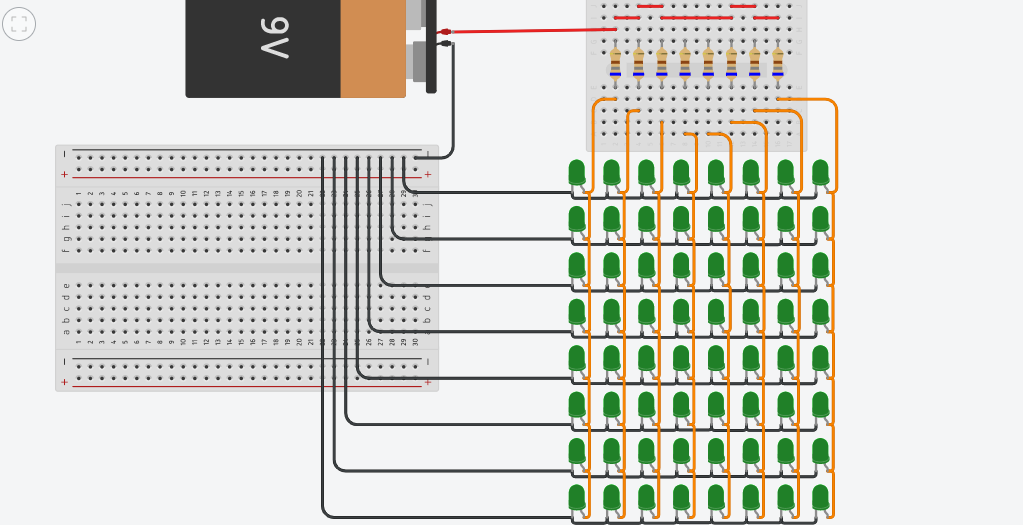
\includegraphics[width=10cm]{1.png}
\centering
\caption{Mariz de leds}
\label{fig:matriz de leds}
\end{figure}

\begin{figure}[h]
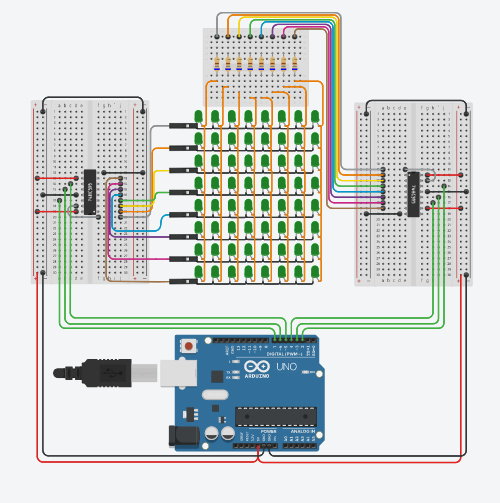
\includegraphics[width=10cm]{2.png}
\centering
\caption{Implementación circuito integrado y arduino}
\label{fig:implementación}
\end{figure}


\begin{figure}[h]
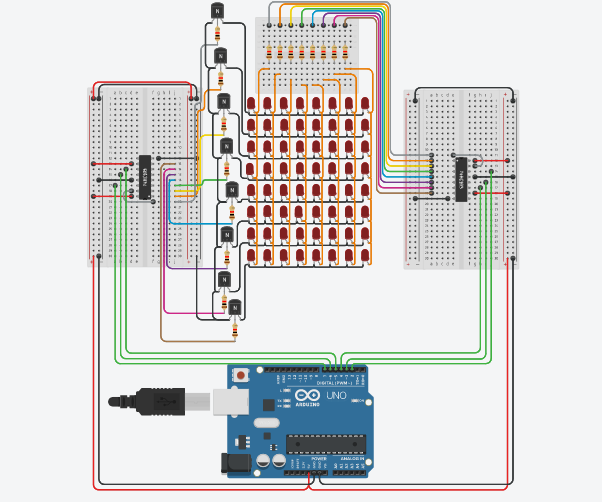
\includegraphics[width=10cm]{circuito finalizado.png}
\centering
\caption{Circuito finalizado}
\label{fig:circuito finalizado}
\end{figure}


\end{document}